\begin{figure}[t]
\vspace{-6mm}
\centering

\vspace{-3mm}
\mbox{
  \subfigure[Computation time for $\sum AB$ using standard algorithm vs our inferred optimal algorithm.]{
      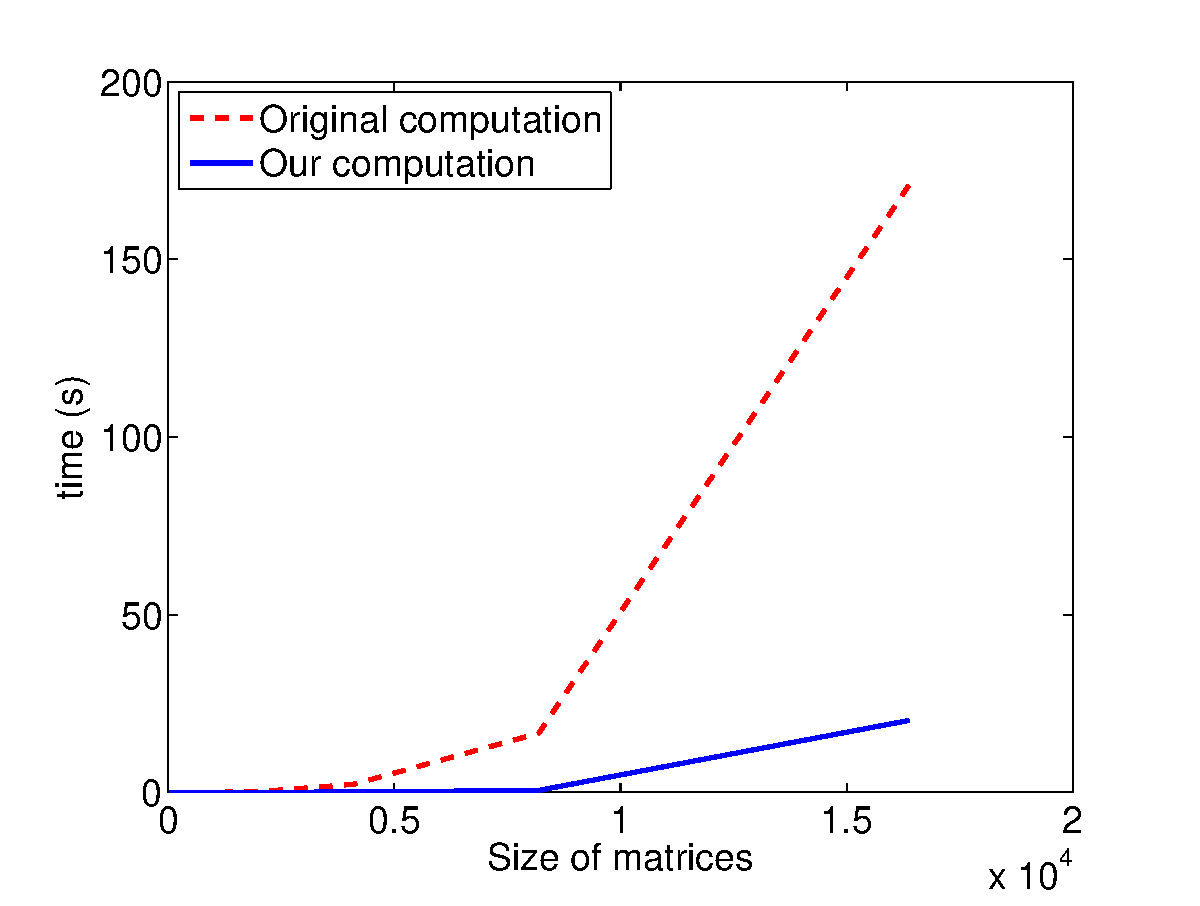
\includegraphics[width=0.55\linewidth]{img/ab.eps}
      \label{ab}
  }\quad
\subfigure[Approximations of $e^x$ using Taylor series.]{
  \includegraphics[width=0.35\linewidth]{img/approximations.eps} 
  \label{approximations}
  }
}
\vspace{-3mm}
\subfigure[Relative approximation error of the partition function for different
degrees of Taylor approximation. Max, mean and min errors are shown for 100
different trials for $W$ of size $ 7 \times 7$, with $W_{ij} \sim
\text{Laplacian}(s)$ and $s=0.05$ (blue) and $s=0.3$ (red).]{
  \includegraphics[scale=0.44]{img/partition_approx_rob.eps}
  \label{error_approx}
}

\subfigure[Comparison of computation time for naive exponential time algorithm vs our optimized derivation.]{
  \includegraphics[scale=0.24]{img/time_approx.eps}
  \label{time_approx}
}
\vspace{-7mm}
\caption{Experimental results.}
\end{figure}
